\documentclass{article}\usepackage[]{graphicx}\usepackage[]{color}
%% maxwidth is the original width if it is less than linewidth
%% otherwise use linewidth (to make sure the graphics do not exceed the margin)
\makeatletter
\def\maxwidth{ %
  \ifdim\Gin@nat@width>\linewidth
    \linewidth
  \else
    \Gin@nat@width
  \fi
}
\makeatother

\definecolor{fgcolor}{rgb}{0.345, 0.345, 0.345}
\newcommand{\hlnum}[1]{\textcolor[rgb]{0.686,0.059,0.569}{#1}}%
\newcommand{\hlstr}[1]{\textcolor[rgb]{0.192,0.494,0.8}{#1}}%
\newcommand{\hlcom}[1]{\textcolor[rgb]{0.678,0.584,0.686}{\textit{#1}}}%
\newcommand{\hlopt}[1]{\textcolor[rgb]{0,0,0}{#1}}%
\newcommand{\hlstd}[1]{\textcolor[rgb]{0.345,0.345,0.345}{#1}}%
\newcommand{\hlkwa}[1]{\textcolor[rgb]{0.161,0.373,0.58}{\textbf{#1}}}%
\newcommand{\hlkwb}[1]{\textcolor[rgb]{0.69,0.353,0.396}{#1}}%
\newcommand{\hlkwc}[1]{\textcolor[rgb]{0.333,0.667,0.333}{#1}}%
\newcommand{\hlkwd}[1]{\textcolor[rgb]{0.737,0.353,0.396}{\textbf{#1}}}%
\let\hlipl\hlkwb

\usepackage{framed}
\makeatletter
\newenvironment{kframe}{%
 \def\at@end@of@kframe{}%
 \ifinner\ifhmode%
  \def\at@end@of@kframe{\end{minipage}}%
  \begin{minipage}{\columnwidth}%
 \fi\fi%
 \def\FrameCommand##1{\hskip\@totalleftmargin \hskip-\fboxsep
 \colorbox{shadecolor}{##1}\hskip-\fboxsep
     % There is no \\@totalrightmargin, so:
     \hskip-\linewidth \hskip-\@totalleftmargin \hskip\columnwidth}%
 \MakeFramed {\advance\hsize-\width
   \@totalleftmargin\z@ \linewidth\hsize
   \@setminipage}}%
 {\par\unskip\endMakeFramed%
 \at@end@of@kframe}
\makeatother

\definecolor{shadecolor}{rgb}{.97, .97, .97}
\definecolor{messagecolor}{rgb}{0, 0, 0}
\definecolor{warningcolor}{rgb}{1, 0, 1}
\definecolor{errorcolor}{rgb}{1, 0, 0}
\newenvironment{knitrout}{}{} % an empty environment to be redefined in TeX

\usepackage{alltt}

\usepackage{fancyhdr} % Required for custom headers
\usepackage{lastpage} % Required to determine the last page for the footer
\usepackage{extramarks} % Required for headers and footers
\usepackage{graphicx} % Required to insert images
\usepackage{hyperref}
\usepackage{amsmath} %for binomial pdf
\usepackage{parskip} % so that there's space bw paragraphs
\usepackage{float}
\usepackage{amsfonts}
\usepackage{verbatim}
\graphicspath{"~/almhub_0823/exp_design/homework/HW4"}



% Margins
\topmargin=-0.45in
\evensidemargin=0in
\oddsidemargin=0in
\textwidth=6.5in
\textheight=9.0in
\headsep=0.25in 

\linespread{1.1} % Line spacing

% Set up the header and footer
\pagestyle{fancy}
\lhead{STAT 541: Experimental Design} % Top left header
\chead{HW 5} % Top center header
\rhead{Andrea Mack} % Top right header
\lfoot{02/24/2017} % Bottom left footer
\cfoot{} % Bottom center footer
\rfoot{Page\ \thepage\ of\ \pageref{LastPage}} % Bottom right footer
\renewcommand\headrulewidth{0.4pt} % Size of the header rule
\renewcommand\footrulewidth{0.4pt} % Size of the footer rule

\setlength\parindent{0pt} % Removes all indentation from paragraphs
\setlength\parskip{0.5cm}
\restylefloat{table}

%----------------------------------------------------------------------------------------
%	DOCUMENT STRUCTURE COMMANDS
%	Skip this unless you know what you're doing
%----------------------------------------------------------------------------------------

% Header and footer for when a page split occurs within a problem environment
\newcommand{\enterProblemHeader}[1]{
\nobreak\extramarks{#1}{#1 continued on next page\ldots}\nobreak
\nobreak\extramarks{#1 (continued)}{#1 continued on next page\ldots}\nobreak
}

% Header and footer for when a page split occurs between problem environments
\newcommand{\exitProblemHeader}[1]{
\nobreak\extramarks{#1 (continued)}{#1 continued on next page\ldots}\nobreak
\nobreak\extramarks{#1}{}\nobreak
}


%----------------------------------------------------------------------------------------%
\IfFileExists{upquote.sty}{\usepackage{upquote}}{}
\begin{document}



\begin{enumerate}

\item
\begin{enumerate}
\item %1

{\it You are told to analyze the experimental results assuming a randomized complete block design (RCBD) was run. Prepare an ANOVA table to test the hypotheses regarding fertilizers. Using an $\alpha$ = .05 level, what do you conclude?}

At the $\alpha$ = 0.05 significance level, based on a p-value less than 0.001 there is strong evidence at least one of the fertilizers had a different true mean percent coverage after accounting for row.

\begin{center}
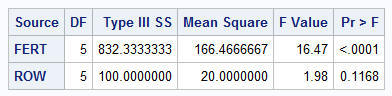
\includegraphics{prob1a}
\end{center}

\item 
{\it (2pt) Perform Tukey's test on the fertilizer means. What do you conclude?}

{\bf Tukey's test for additivity or Tukey's family-wise correction for multiple comparisons?}

At the 95\% family wise confidence level using Tukey's adjustment for multiple comparisons, there is strong evidence after accounting for row, average percent coverage from plots with fertilizer E are lower than plots with fertilizers C, A, and D. Similarly, there is strong evidence average percent coverage from plots with fertilizer F are lower than plots with fertilizers A and D and strong evidence average percent coverage from plots with fertilizer C is lower than plots with fertilizer A.

\begin{center}
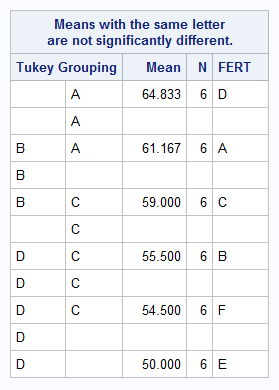
\includegraphics{prob1b}
\end{center}

\item 
{\it (1pt) Make a normal probability plot of the residuals and a plot of residuals vs predicted values. Comment on the results.}

The residuals vs. predicted plot shows more variability in the center than on the edges, particularly with residuals ranging from 4 to -6 in the center of the plot and ranging from around -2 to 2 on the edges of the plot.

\begin{center}
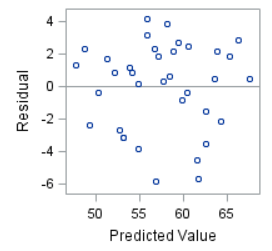
\includegraphics{prob1c}
\end{center}

{\bf CODE FOR RCBD ANALYSIS}

\begin{verbatim}
PROC GLM DATA=in PLOTS = (ALL);
CLASS row fert;
MODEL cover = fert row / SS3 SOLUTION;
MEANS rows;
MEANS fert / TUKEY CLDIFF LINES;
RUN;
\end{verbatim}

\item
{\it (5pt) Unfortunately, the experiment was set up by another researcher who used a a latin square design with plot column as the second blocking variable. Reanalyze the data as a latin square design by answering questions (a), (b), and (c) again.}

a)

At the $\alpha$ = 0.05 significance level using a latin squares design, based on a p-value less than 0.001 there is strong evidence at least one of the fertilizers had a different true mean percent coverage after accounting for row.

\begin{center}
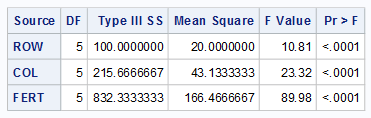
\includegraphics{latin1a}
\end{center}

b)

At the 95\% family-wise confidence level using Tukey's multiple comparison adjustment, with a latin squares design analysis, there was strong evidence the true mean percent coverage from plots with fertilizer E was lower than the true mean covereage from plots fertilized with all other fertilizers. Similarly, there was strong evidence the true mean percent coverage from plots with fertilizer F was lower than the true mean covereage fro plots with fertilizers C, A, and D. There was strong evidence the true mean percent coverage from plots fertilized with fertilier C was lower than the true mean percent coverage from plots fertilized with fertilizer D. There was strong evidence the true mean percent coverage for plots fertilized with fertlizer D was higher than all that from plots fertilized with all other fertilizers.

\begin{center}
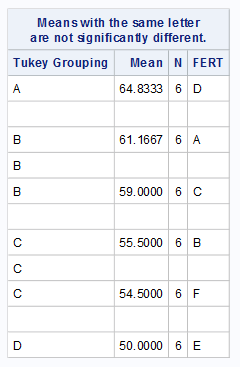
\includegraphics{latin1b}
\end{center}

c)

Though at first glance we see more variation in the center of the residuals than on the edges, looking closer we notice the scale of the residual axis only goes between roughly 2 and -2. While non-constant variance is present, the degree is small as signified by the scale of the residual axis.

\begin{center}
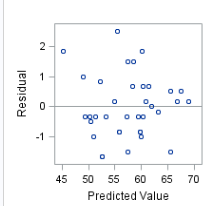
\includegraphics{latin1c}
\end{center}



{\bf CODE FOR LATIN SQUARES ANALYSIS}

\begin{verbatim}
proc glm data = in plots = (all);
class row col fert;
model cover = row col fert /ss3;
means row col;
means fert /tukey alpha=0.05;
output out=diag p=pred r=resid;
title 'LATIN SQUARES ANALYSIS';
run;
\end{verbatim}

\item
{\it (1pt) Identify any significant changes that occurred between analyses.}

Significant changes occured in the multiple comparisons and in the residuals vs. predicted plots. HOV is more reasonably met in the latin squares analysis, and noteable fertlizers D and E resulted in significant difference in mean percent coverage from all other fertilizers.

\item 
{\it (2pt) Calculate the row block and column block means. In terms of a physical context, interpret any patterns (if they exist) across the row and column means.}

It appears that moving down the rows from 1 to 6 the mean percent coverage increases, as does the row standard deviation with a slight deviation from the increasing pattern.

Column means decrease from columns 4 to 6 and column standard deviations are smallest on the edges (1 and 6) and increase towards the center, being most variable.

{\bf What other physical to go off of?}

\begin{figure}
\centering
\begin{minipage}{.5\textwidth}
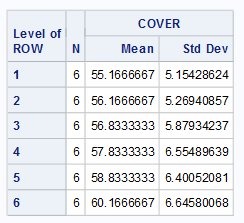
\includegraphics{row1}
\end{minipage}%
\begin{minipage}{.5\textwidth}
\centering
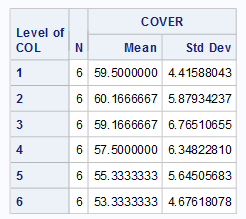
\includegraphics{col1}
\end{minipage}
\end{figure}

\end{enumerate}
\item %2

\end{enumerate}
\end{document}
